\documentclass[conference]{IEEEtran}
\IEEEoverridecommandlockouts
% The preceding line is only needed to identify funding in the first footnote. If that is unneeded, please comment it out.
\usepackage{cite}
\usepackage{amsmath,amssymb,amsfonts}
\usepackage{algorithmic}
\usepackage{graphicx}
\usepackage{textcomp}
\usepackage{xcolor}
\usepackage{caption}
\usepackage{subcaption}
\usepackage{array}

\usepackage{mathtools} 

%added by Ye
\usepackage{fontspec}

%for phonetic symbol
\usepackage{tipa}
%for Greek letter
%\usepackage{textgreek}

%for typing Myanmar text, you can also used with Myanmar3 font
\newfontfamily {\padauktext}[Script=Myanmar]{Padauk}
%\newfontinstance {\padauktext}[Script=Myanmar]{Padauk}

%for double quote
\newcommand{\quotes}[1]{``#1''}

%for scalability of all sizes of paper
\renewcommand{\baselinestretch}{0.99}
%added by Ye

\usepackage{tabularx}

\def\BibTeX{{\rm B\kern-.05em{\sc i\kern-.025em b}\kern-.08em
    T\kern-.1667em\lower.7ex\hbox{E}\kern-.125emX}}
\begin{document}

\title{Mon Language and Culture}

\author{\IEEEauthorblockN{1\textsuperscript{st} Ye Kyaw Thu}
\IEEEauthorblockA{\textit{Language and Semantic Technology Research Team (LST)} \\
\textit{National Electronics and Computer Technology Center (NECTEC)}\\
PathumThani, Thailand \\
ka2pluskha2@gmail.com}
\and
\IEEEauthorblockN{2\textsuperscript{nd} Htet Htet Yadanar Oo}
\IEEEauthorblockA{\textit{Faculty of Information Science} \\
\textit{University of Technology (Yatanarpon Cyber City)}\\
Pyin Oo Lwin, Myanmar \\
htetyadana123@gmail.com}
}

\maketitle

\begin{abstract}
This article is about Mon language, spoken in southeastern Burma and western Thailand. The Mon language ({\padauktext /moʊn/}, Mon: {\padauktext ဘာသာ မန်}; Burmese: {\padauktext မွန်ဘာသာ}) is an Austroasiatic language spoken by the Mon people, who live in Myanmar and Thailand. Mon, like the related Khmer language or Vietic languages, but unlike most languages in mainland Southeast Asia, is not tonal. In recent years, usage of Mon has declined rapidly, especially among the younger generation. Many ethnic Mon in Myanmar are monolingual in Burmese, and the language is classified as "vulnerable" by UNESCO. The current number of speakers is approximately 800,000 in 2007. In Myanmar, the majority of speakers live in Mon State, followed by Tanintharyi Region and Kayin State. Mon was first written during the 6th century AD in two different scripts: one derived from the Grantha script, and one derived from the Kadamba or Grantha script. The Mon script first appeared in the Mayzedi inscriptions in 1113
\end{abstract}

\begin{IEEEkeywords}
Mon Language and Scripts, Mon people and culture
\end{IEEEkeywords}

\section{General Information}
Mon is an Austroasiatic language spoken in parts of Myanmar/Burma and Thailand. In 2004 there were 850,000 speakers, mainly in Mon State, and also in the Tanintharyi Region and Kayin State in southern Myanmar. The language was widely spoken in southern Burma until the middle of the 19th century, when the area was taken over by the British. After then large numbers of people migrated to the area from India and China, and Mon became marginalized. The symbol of the Mon people is the hongsa (Mon: {\padauktext ဟံသာ}, [hɔŋsa]), a mythological water bird that is often illustrated as a swan. It is commonly known by its Burmese name, hintha (Burmese: {\padauktext ဟင်္သာ}, IPA: [hɪ́ɴθà]) or its Thai name: hong. \cite{b1} The Mon assimilated to Thai culture long ago, yet the royal women of the Chakri dynasty perform and keep their Mon heritage alive in the Thai court. The western Mon of Myanmar were largely absorbed by Bamar society. They have worked to preserve their language and culture and to regain a greater degree of political autonomy. In the Mon language, the Mon are known as the Mon (spelt {\padauktext မောန်} or {\padauktext မန်} and pronounced /mòn/), based on the Pali term Rāmañña ({\padauktext ရာမည}), which refers to the Mon heartland along the Burmese coast. In classical Mon literature, they are known as the Raman ({\padauktext ရာမန်}). The language was widely spoken in southern Burma until the middle of the 19th century, when the area was taken over by the British. After then large numbers of people migrated to the area from India and China, and Mon became marginalized.

\section{Mon People and Mon Culture}
Mon State (Burmese: {\padauktext မွန်ပြည်နယ်}, pronounced [mʊ̀ɴ pjìnɛ̀]; Mon: {\padauktext တွဵုရးဍုၚ်မန်၊ ရာမညဒေသ}) is an administrative division of Myanmar. It lies between Kayin State to the east, the Andaman Sea to the west, Bago Region to the north and Tanintharyi Region to the south, also having a short border with Thailand's Kanchanaburi Province at its south-eastern tip. The Mon were a major source of influence on the culture of Myanmar and the culture of Thailand.\\
\par Mon culture and traditional heritages includes spiritual dances, musical instruments such as the kyam or "crocodile xylophone", the saung harp and a flat stringed instrument. Mon dances are usually played in a formal theater or sometimes in an informal district of any village. The dances are followed by background music using a circular set of tuned drums and claps, crocodile xylophone, gongs, flute, flat guitar, harp, etc. Mon in Burma wear clothes similar to the Bamars. Those living in Thailand have adopted Thai style scarfs and skirts. Mon cuisines and culinary traditions have had significant influences on the Burmese cuisine and Central Thai cuisine today. For example, Htamanè ({\padauktext ထမနဲ}) and Thingyan Htamin ({\padauktext သင်္ကြန်ထမင်း}). A traditional Mon dish ({\padauktext သင်္ကြန်ထမင်း}) served with rice soaked with cool candle-and-jasmine-scented water is consumed by the Mon people during the Thingyan (Songkran) Festival in the summer.

\begin{figure}[h!]
  \centering
  \begin{subfigure}[b]{0.4\linewidth}
    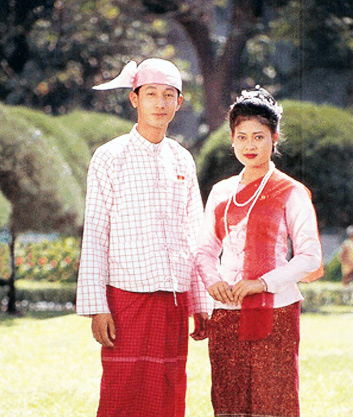
\includegraphics[width=\linewidth, height=3.5cm]{./fig/mon.jpg}
    \caption{Mon Traditional \\Costume}
  \end{subfigure}
  \begin{subfigure}[b]{0.4\linewidth}
    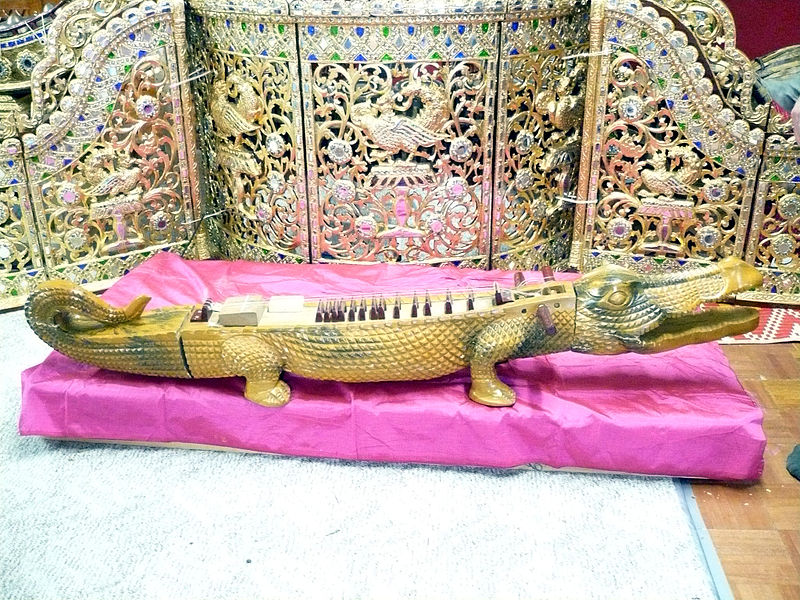
\includegraphics[width=\linewidth, height=3.5cm]{./fig/saung.jpg}
    \caption{Kyan or Crocodile Xylophone}
  \end{subfigure}
  \begin{subfigure}[b]{0.4\linewidth}
    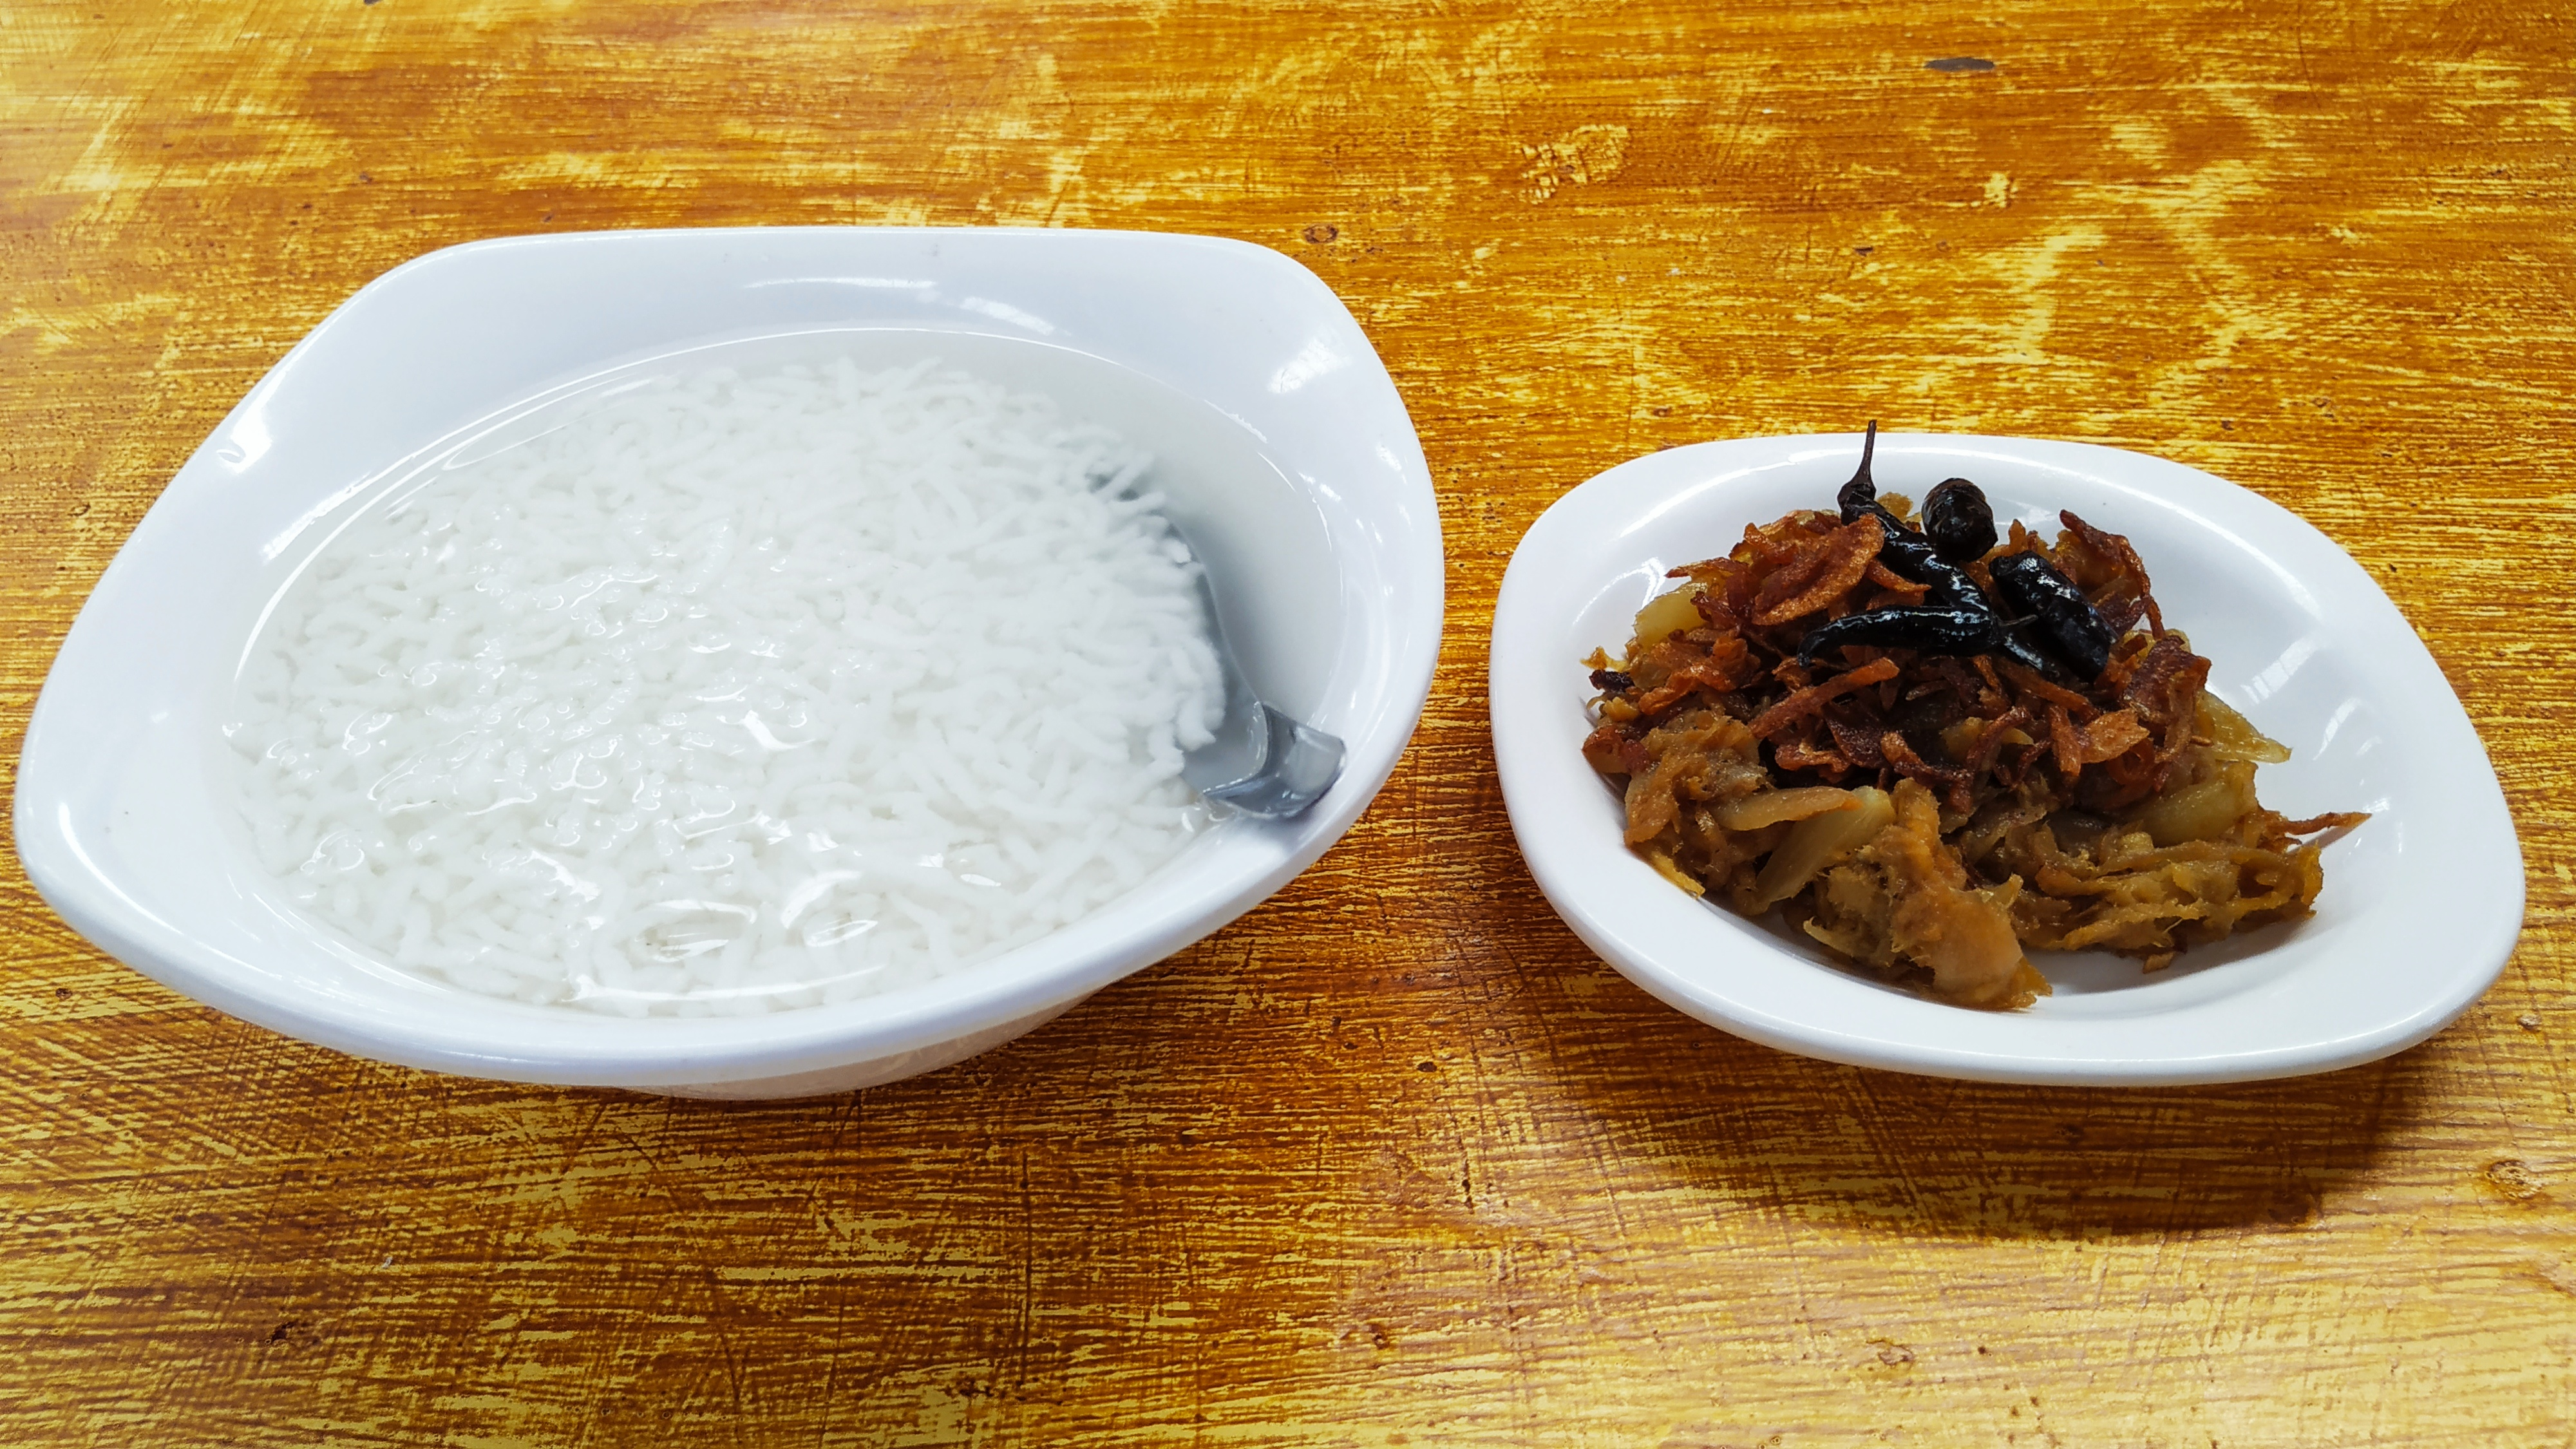
\includegraphics[width=\linewidth, height=3.5cm]{./fig/thingyan.jpg}
    \caption{Thingyan Htamin ({\padauktext သင်္ကြန်ထမင်း})}
  \end{subfigure}
  \begin{subfigure}[b]{0.4\linewidth}
    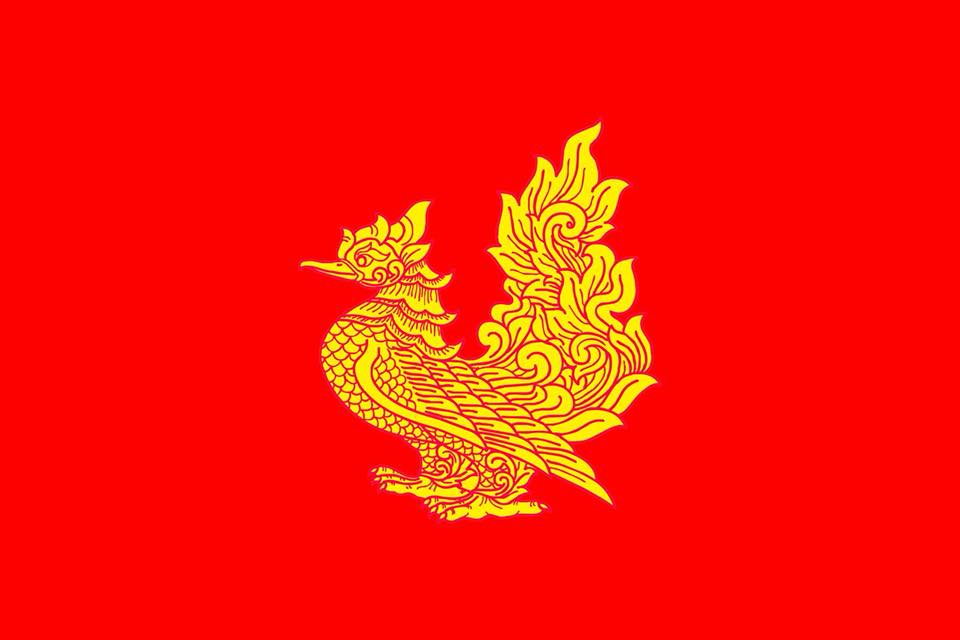
\includegraphics[width=\linewidth, height=3.5cm]{./fig/hinthar.jpg}
    \caption{The Symbol of Mon (Hin Thar)}
  \end{subfigure}
  \caption{Mon Traditional Culture}
  \label{fig:coffee}
\end{figure}

\section{History}
The Mon are the earliest known inhabitants of lower Burma. They founded an empire, and introduced both writing and Buddhism into Burma. In the year 573, two Mon brothers, Prince Samala and Prince Wimala, founded the Mon kingdom Hongsavatoi at the present site of modern Pegu. This kingdom flourished in peace and prosperity for several centuries until it was occupied by the Burman dynasty. In 1757, the Burma ruler U Aungzeya invaded and devastated the Mon kingdom, killing tens of thousands of Mon, including learned Mon priests, pregnant women, and children. Over 3,000 priests were massacred by the victorious Burmans in the capital city alone. Thousands more priests were killed in the countryside. The surviving priests fled to Thailand, and Burman priests took over the monasteries. Most of the Mon literature, written on palm leaves, was destroyed by the Burmans. Use of the Mon language was forbidden, and Burman became the medium of instruction. Mon people were persecuted, oppressed, and enslaved, and countless people were burned in holocausts, like the Jews before the Nazis. Mon properties and possessions were looted and burned throughout Burma. Mons fled further south into Burma's Tenasserim Division and east into Thailand. Unfortunately, the oppression of the Mon people has persisted to the present day.\cite{b2}

\begin{figure}[h!]
  \centering
  \begin{subfigure}[b]{0.4\linewidth}
    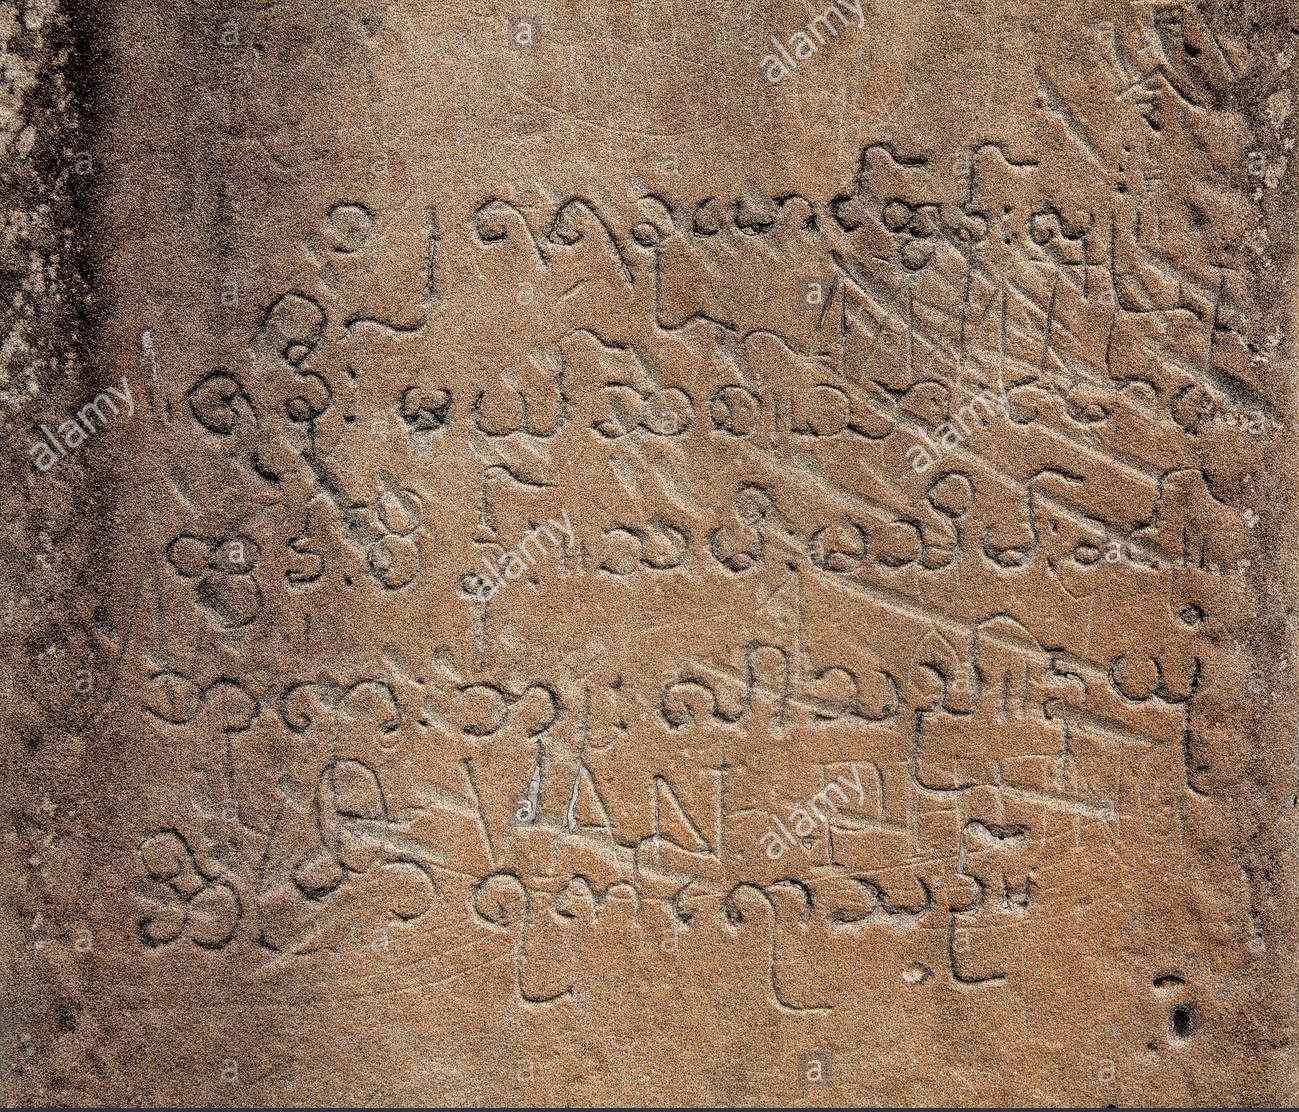
\includegraphics[width=\linewidth, height=3.9cm]{./fig/his1.jpg}
    \caption{Stone Piller of \\Mon Language}
  \end{subfigure}
  \begin{subfigure}[b]{0.4\linewidth}
    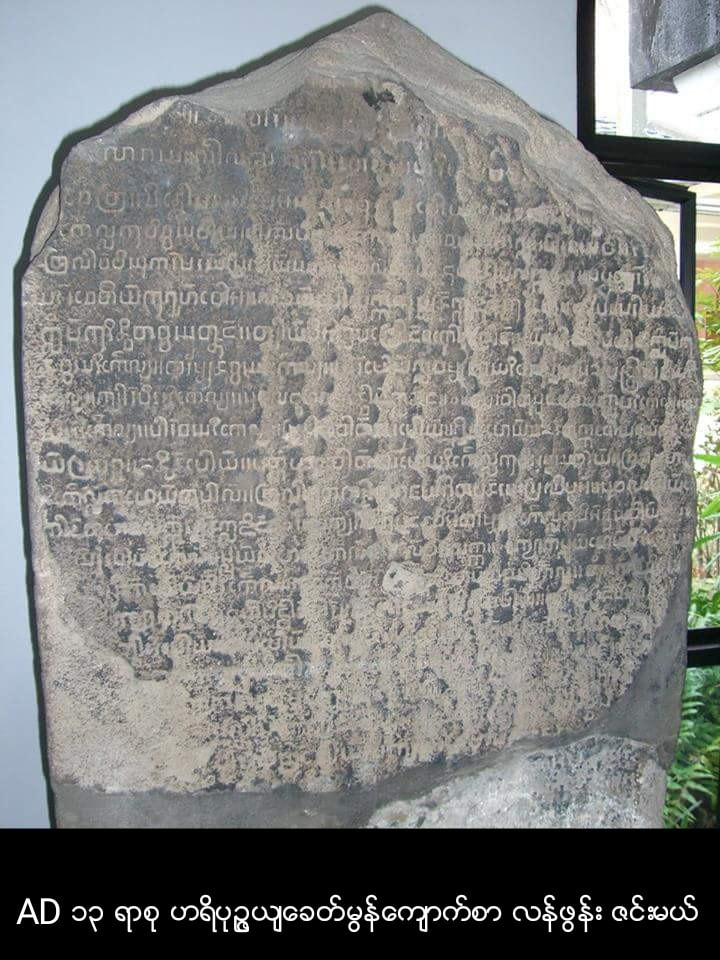
\includegraphics[width=\linewidth, height=3.7cm]{./fig/his3.jpg}
    \caption{{\padauktext AD၁၃ရာစု ဟရိပုဉ္ဇယျ\\ခေတ်မွန်ကျောက်စာ}}
  \end{subfigure}
  \caption{History of Mon Language}
  \label{fig:coffee}
\end{figure}

\section{Mon Language and Scripts}
\label{sec:Mon Language}
The Mon language is part of the Monic group of the Austroasiatic languages (also known as Mon–Khmer language family), closely related to the Nyah Kur language and more distantly related to Khmer. The writing system is based on Indic scripts. The Mon language is one of the earliest documented vernacular languages of Indochina. Burmese language also has a lot of words derived from or borrowed from the Mon language, especially related with administration, architecture, cloth, cuisine and flowers.

\subsection{Alphabet}
\label{subsec:Mon Alphabet}
The Mon script is basically a syllabic system. Vowel signs are added to the front, back, bottom or top of the consonant signs. The original values of many letters  have  changed  during  the  recorded history  of  the  Mon  language, while  the  spelling has hardly been adjusted. The present day situation is therefore similar to the one of Englsih, where there is a great discrepancy between the written and the spoken forms  of  the  language. Although the Mon and Burmese writing systems are basically the same, Mon is more complex,  making  use  of more superscript consonants. \cite{b4} The Mon alphabet contains 35 consonants shown in Table 1.
\par Mon uses the same diacritics and diacritic combinations as in Burmese to represent vowels, with the addition of a few diacritics unique to the Mon script, including {\padauktext ဴ }(/ɛ̀a/), and {\padauktext ဳ} (/i/), since the diacritic {\padauktext ိ} represents /ìˀ/.[18] Also, {\padauktext ဨ } (/e/) is used instead of {\padauktext ဧ }, as in Burmese. There are 31 vowels in Mon Language; 6 independent vowels and 25 vowel diacritics (shown in Table 2). Moreover, there are 9 medials ({\padauktext ၚ  }, {\padauktext ၞ  },, {\padauktext ၟ  }, {\padauktext ျ }, {\padauktext ြ }, {\padauktext ၠ  }, {\padauktext ွ  }, {\padauktext ှ  }, {\padauktext ်  }). In Mon script, ``{\padauktext ၊ }'' is used for a comma, and ``{\padauktext ။ }'' is used for a period.\cite{b5}

\begin{table}
\begin{center}
\caption{\label{Mon Alphabet Table} Mon Alphabet (Consonant) }
\normalsize %set fontsize in table
\begin{tabular}{ |m{1cm}|m{1cm}|m{1cm}|m{1cm}|m{1cm}| }
\hline
{\padauktext က} & {\padauktext ခ} & {\padauktext ဂ} & {\padauktext ဃ} & {\padauktext \color{red}ၚ} \\ 
{Ka} & {Kha} & {Gé} & {Khé} & \color{red}{Ngé} \\
\hline
{\padauktext စ} & {\padauktext ဆ} & {\padauktext ဇ} & {\padauktext \color{red}ၛ} & {\padauktext ည} \\ 
{Ja} & {Cha} & {Jé} & {\color{red}Ché} & {Nyé} \\
\hline
{\padauktext ဋ } & {\padauktext ဌ} & {\padauktext ဍ} & {\padauktext ဎ} & {\padauktext ဏ} \\ 
{Ta} & {Tha} & {Da} & {Thé} & {Na} \\
\hline
{\padauktext တ} & {\padauktext ထ} & {\padauktext ဒ} & {\padauktext ဓ} & {\padauktext န} \\ 
{Ta} & {Tha} & {Dé} & {Thé} & {Né} \\
\hline
{\padauktext ပ} & {\padauktext ဖ} & {\padauktext ဗ} & {\padauktext ဘ} & {\padauktext မ} \\ 
{Pa} & {Pha} & {Bé} & {Phé} & {Mé} \\
\hline
{\padauktext ယ} & {\padauktext ရ} & {\padauktext လ} & {\padauktext ဝ} & {\padauktext သ} \\ 
{Yé} & {Ré} & {Lé} & {Wé} & {Sa} \\
\hline
{\padauktext ဟ} & {\padauktext ဠ} & {\padauktext \color{red}ၜ} & {\padauktext အ} & {\padauktext \color{red}ၝ} \\ 
{Ha} & {La} & \color{red}{Ba} & {Aa} & \color{red}{Bé} \\
\hline
\end{tabular}
\end{center}
\end{table}

\begin{table}
\caption{\label{Mon Vowel Table} Mon Alphabet (Vowel) }
\begin{tabularx}{0.45\textwidth} { 
  | >{\raggedright\arraybackslash}X 
  | >{\centering\arraybackslash}X 
  | >{\raggedleft\arraybackslash}X | }
 \hline
 \bf Initial or independent symbol  & \bf diacritic  & \bf Transcription and notes  \\
\hline
 {\padauktext အ} & none, inherent vowel & a or a or e - /a/, /ɛ̀/ after some consonants \\
 \hline
 {\padauktext အာ}  & {\padauktext ာ}  & ā-spelled as ါ to avoid confusion with certain letters  \\
 \hline
 {\padauktext ဣ}  & {\padauktext ိ}  & i  \\
\hline
 {\padauktext ဣီ}  & {\padauktext ီ}  & ī or oe - /ì/, /ɔe/ after some consonants   \\
\hline
 {\padauktext ဥ}  & {\padauktext ု}  & u  \\
\hline
 {\padauktext ဥူ}  & {\padauktext ူ}  & ū or ao - /ù/, /ao/ after some consonants   \\
\hline
 {\padauktext ဨ}  & {\padauktext ေ}  & e  \\
\hline
 {\padauktext အဲ}  & {\padauktext ဲ}  & ai  \\
\hline
 {\padauktext အော}  & {\padauktext ော}  & o - spelled as ေါ to avoid confusion with certain consonants.  \\
\hline
 {\padauktext အဴ‌‍‍}  & {\padauktext ဴ} & āi/oi\\
\hline
 {\padauktext အံ}  & {\padauktext ံ}  & òm  \\
\hline
 {\padauktext အး}  & {\padauktext း}  & ah  \\
\hline
\end{tabularx}
\end{table}

\par Other diacritic vowels and transcription notes are as in the following:
\begin{itemize}
\item {\padauktext ို} \textrightarrow \: iu
\item {\padauktext ာံ} \textrightarrow \:  	āṃ
\item {\padauktext ုံ} \textrightarrow \: uṃ
\item {\padauktext ေံ} \textrightarrow \: eṃ
\item {\padauktext ောံ} \textrightarrow \:  	oṃ
\item {\padauktext ီ} \textrightarrow \:  	aṁ
\item {\padauktext ီု} \textrightarrow \: uṁ
\item {\padauktext ာဲ} \textrightarrow \:  	āai
\item {\padauktext ုဲ} \textrightarrow \: uai
\item {\padauktext ေဲ} \textrightarrow \: eai
\item {\padauktext ောဲ} \textrightarrow \: oai
\item {\padauktext ိုဲ} \textrightarrow \: iuai
\item {\padauktext ဵု} \textrightarrow \: uew
\end{itemize}

\subsection{Dialects}
\label{subsec:Mon Dialects}
Mon has three primary dialects in Burma, coming from the various regions the Mon inhabit. They are the Central (areas surrounding Mottama and Mawlamyine), Bago, and Ye dialects.[10] All are mutually intelligible. Thai Mon has some differences from the Burmese dialects of Mon, but they are mutually intelligible. Ethnologue lists Mon dialects as Martaban-Moulmein (Central Mon, Mon Te), Pegu (Mon Tang, Northern Mon), and Ye (Mon Nya, Southern Mon), with high mutual intelligibility among them.\cite{b3}

\subsection{Grammar of Myanmar and Mon Sentence}
\label{subsecsec:Grammar}
Both Burmese and Mon make extensive use of (partly) grammaticalized secondary verbs to express a wide range of functions, including aspect, modality, directionality, manner, and others. A number of these secondary verbs are common to Mon and Burmese in some or all their functions, like postverbal ‘get’, yá in Burmese and kɤ̀ʔ in Mon, which is used to express general deontic possibility in both languages (as well as many other Southeast Asian languages, see Enfield 2003). The verb meaning ‘win’, Burmese nain, Mon màn, expresses epistemic possibility in both languages. Besides, the numerous common grammaticalisations, Mon and Burmese go separate ways in many instances. In some cases, southern Burmese differs from standard Burmese in a way that brings it closer to Mon, as illustrated in the following examples.[9]
\noindent mon: {\padauktext ဍေံ လဴ စကဵု အဲ ။}\\
my:  {\padauktext သူငါ့ကိုပြောတယ်။}\\
eng: He told me .\\

\noindent mon: {\padauktext ဗှ်ေဟွံဒးအာရ။}\\
my:  {\padauktext သွားမပြောထိတော့ဘူး ။}\\
eng: You don’t have to go any more.\\

\noindent mon: {\padauktext လိက်အဲဂှ် အဲချူကေတ်။}\\
my:  {\padauktext ကျွန်တော့် စာကို ကျွန်တော် ရေးယူမယ်။။}\\
eng: I will write my text myself. \\

\noindent mon: {\padauktext ဍေံ ဟီု အေရဝ်ေသံ ဟွံလေပ်ပုဟ်။}\\
my:  {\padauktext သူ ထိုင်းစကားမပြောတတ်ဘူး ။}\\
eng: He cannot speak Thai Language. \\

\noindent mon: {\padauktext အဲကဵုဍေံလိက်။}\\
my:  {\padauktext ငါသူ့ကို စာအုပ်ပေးခဲ့ပါတယ် ။}\\
eng: I gave him book. \\

\subsection{Phonology}
In the Mon script, consonants belong to one of two registers: clear and breathy, each of which has different inherent vowels and pronunciations for the same set of diacritics. For instance, {\padauktext က}, which belongs to the clear register, is pronounced /kaˀ/, while {\padauktext ဂ} is pronounced /ɡɛ̀ˀ/, to accommodate the vowel complexity of the Mon phonology. The addition of diacritics makes this obvious. Whereas in Burmese, spellings with the same diacritics are rhyming, in Mon, this depends on the consonant's inherent register. A few examples are listed below:\cite{b7}
\begin{itemize}
\item {\padauktext က} +{\padauktext ီ} \textrightarrow {\padauktext ကီ} , pronounced /kɔe/
\item {\padauktext ဂ} +{\padauktext ီ} \textrightarrow {\padauktext ဂီ} , pronounced /kì/
\item {\padauktext က} +{\padauktext ူ} \textrightarrow {\padauktext ကူ} , pronounced /kao/
\item {\padauktext ဂ} +{\padauktext ူ} \textrightarrow {\padauktext ဂူ} , pronounced /kù/
\end{itemize}

Mon uses the same diacritics and diacritic combinations as in Burmese to represent vowels, with the addition of a few diacritics unique to the Mon script, including {\padauktext ဴ }(/ɛ̀a/), and {\padauktext ဳ }(/i/), since the diacritic {\padauktext ိ }represents /ìˀ/.[11] Also,{\padauktext ဨ }(/e/) is used instead of{\padauktext ဧ}, as in Burmese. The Mon language has 8 medials, as follows:{\padauktext ္ၚ} (/-ŋ-/),{\padauktext ၞ} (/-n-/),{\padauktext ၟ }(/-m-/),{\padauktext ျ }(/-j-/),{\padauktext ြ} (/-r-/),{\padauktext ၠ} (/-l-/),{\padauktext ွ} (/-w-/), and{\padauktext ှ} (/-hn-/). Consonantal finals are indicated with a virama {\padauktext(်)}, as in Burmese. Furthermore, consonant stacking is possible in Mon spellings, particularly for Pali and Sanskrit-derived vocabulary.\cite{b6}

\begin{table}
\begin{center}
\caption{\label{Mon Phonology Consonant} Phonology consonant }
\normalsize %set fontsize in table
\begin{tabular}{ |m{1.5cm}|m{1cm}|m{1cm}|m{1cm}|m{1cm}|m{1cm}| }
\hline
 & Bilabial & Dental & Palata & Velar & Glottal \\
\hline
Stops & p p\textsuperscript{h} ɓ & t t\textsuperscript{h} ɗ & c c\textsuperscript{h} & k k\textsuperscript{h} & \textipa{\: ?} \\
\hline
Fricatives &  & s & ç\textsuperscript{1} &  & h \\
\hline
Nasals & m & n & ɲ & ŋ &  \\
\hline
Sonorants & w & l,r & j &  &  \\
\hline

\end{tabular}
\end{center}
\end{table}

\begin{table}
\begin{center}
\caption{\label{Mon Phonology Vowels} Phonology vowels }
\normalsize %set fontsize in table
\begin{tabular}{ |m{2cm}|m{1.2cm}|m{1.3cm}|m{1cm}| }
\hline
 & Font & Central & Back \\
\hline
Close & i &  & u \\
\hline
Close-mid & e & ə & o \\
\hline
Open-mid & ɛ & ɐ & c  \\
\hline
Open &  & a & c \\
\hline

\end{tabular}
\end{center}
\end{table}
/ç/ is only found in Burmese loans. Unlike the surrounding Burmese and Thai languages, Mon is not a tonal language. As in many Mon–Khmer languages, Mon uses a vowel-phonation or vowel-register system in which the quality of voice in pronouncing the vowel is phonemic. There are two registers in Mon:

\begin{enumerate}
  \item Clear (modal) voice, analyzed by various linguists as ranging from ordinary to creaky
  \item Breathy voice, vowels have a distinct breathy quality
\end{enumerate}
One study involving speakers of a Mon dialect in Thailand found that in some syllabic environments, words with a breathy voice vowel are significantly lower in pitch than similar words with a clear vowel counterpart.[23] While difference in pitch in certain environments was found to be significant, there are no minimal pairs that are distinguished solely by pitch. The contrastive mechanism is the vowel phonation. In the examples below, breathy voice is marked with a grave accent.\cite{b8}

\section{Mon as Recipient Language}
\label{sec:Mon as recipient language}
With the receding political and economic influence of the Mon people, the Mon language has gradually turned from donor to recipient language. In Myanmar this process can be observed in the development from Old Mon to Middle Mon. As there are next to no Mon documents in Thailand from the time after the arrival of Tai speakers in the Chao Phraya plain, not much can be said about the situation in Thailand in pre-modern times.

\subsection{Thai Influence in Mon}
With no documents illustrating the development of Mon in Thailand after the Tai/Thai expansion, at least at the present stage of research, I will in this section restrict myself to giving some examples of Thai influence in modern Mon varieties spoken in central Thailand as well as some cases of Thaiisms found in Mon literature in Thailand. While these communities were able to maintain their language and customs as different from the surrounding Thai villages and towns, even in the greater Bangkok area, until well into the 20th century (cf. for example Smithies 1986, Foster 1986), heavy structural influence from Thai can be observed in all Mon dialects in Thailand.
\par Today, not many children grow up speaking Mon and also the adults still maintaining their language can be classified as semi-speakers. In this socio-politico-cultural context of assimilation, it is inevitable that many Thai features are found in Mon, either as direct lexical loans, semantic calques, or syntactic replications. The corresponding Thai and Myanmar Mon expressions are in the following: \cite{b9}

\noindent mon: {\padauktext အဲ ဏီအောဂွံ စ ။}\\
thai:  ʨənɔ mə sà yá θè bù.\\
my: {\padauktext ငါ ဘာမှမစားရသေးဘူး ။}\\

\noindent mon: {\padauktext ဂွံမိင်ဗရု ကောန်ၚာ်မဟ ။}\\
thai:  kɤ̀ʔ mòɲ hərùʔ krɔ̀p tɛ̀ərəkaʔ mɛ̀ʔ hɒm.\\
my: {\padauktext သူတို့ကလေးငိုသံကြားကြတယ် ။}\\

\noindent mon: {\padauktext အာတ်ကဵုဗိုလ်လဗးသရာဲ စိင်ချေံ။}\\
thai:  ʔat kɒ pɤ̀ ləpɛ̀h səray coɲ khyɛh.\\
my: {\padauktext ကျုပ်တို့ကို စစ်သည် ၊ ဆင်၊ မြင်း လုံလုံလောက်လောက် ပေးပါ ။}\\

\subsection{Burmese Influence in Mon}
Mon in Myanmar is much more viable than in Thailand, with probably close to a million active speakers, some 25 percent of whom claim to be literate in Mon. Children in many villages in southern Myanmar still grow up with Mon as their first language, learning Burmese only later when they attend Burmese government schools. There is also a substantive literary activity in Mon State, producing a wide range of publications, both printed and other, in Mon.
\par Not only are there numerous Burmese loans and loan translations in Mon, also Mon syntax has converged toward Burmese to a large extent. This convergence leads to some interesting results, as the two languages are typologically very different. In many cases it can be shown that Burmese did not actually introduce new patterns into Mon syntax, but rather helped to activate or strengthen minor use patterns pre-existant in the language. Very often these patterns only superficially correspond to Burmese constructions, which was obviously good enough to treat them as parallel. The following examples illustrate some of the syntactic features listed above.
Sentences (39) to (42) are taken from Mi Kon Plem, a story written in colloquial Mon and published in Moulmein in 2001.
\begin{enumerate}
\item {\padauktext မုဂွံ နင်မုရောကောန်။ } \\
mùʔ  kɤ̀ʔ  nɛ̀ŋ      mùʔ  rao kon. \\
what get CAUS.come what Q   child \\
What did you get, my child?

\item {\padauktext ဂွံ ၚုဟ်မွဲနၜာဒေ ကဝ်ေတှ် သွံ ဏောင်။ } \\
kɤ̀ʔ  ŋùh  mùə nɛ̀ʔ    ɓa  həke   teh,      sɒʔ  noŋ. \\
get price one basket two tical TOP > COND sell ASRT \\
If I get two tical a basket, I’ll sell it.

\item {\padauktext ညးၜာဂှ် နကဵု သွံ ရာန်ေသၞ ဝ်ေကဝ်တုဲ ဂယို င်တဴလမျီု။ } \\
ɲèh    ɓa  kɔ̀h  nɛ̀ʔ   kɒ  sɒʔ  ràn həne.ke    toə, \\
person two MEDL INSTR OBL sell buy vegetables finish \\
həyàŋ     tao  pəyɤ̀m. \\
CAUS.live stay life \\
The two of them sustained their lives by selling vegetables.

\item {\padauktext ညးၜာကဵုတြုဟ်ကဵုဗြဲဂှ် ကောန်ဇာတ်ေရာဟွံ ကလိ ဂွံ ရ ။} \\
ɲèh    ɓa  kraoh kɒ  prèə  kɔ̀h  kon.càt mùə rao hùʔ kəlɒəʔ.kɤ̀ʔ raʔ.\\
person two man   OBL woman MEDL child   one TOP  NEG   get     FOC \\
The man and the woman did not have any children.
\end{enumerate}

\section{Status of Mon Language Today}
\noindent \textbf {Population}: 743,000 in Myanmar (2004), decreasing. Population total all countries: 851,000.
Ethnic population: 1,000,000. \\
\noindent \textbf {Location}: Mon State and Kayin State; also in northern Tanintharyi region. \\
\noindent \textbf {Language} Status: 5 (Developing) [UNESCO: vulnerable] \\
\noindent \textbf {Dialects}: Martaban/Moulmein (Central Mon, Mon Te), Pegu (Mon Tang, Northern Mon), Ye
(Mon Nya, Southern Mon). Intelligibility between Mon varieties high; between Mon in Thailand and Myanmar 99\% (Huffman 1976). Varieties in Myanmar and Thailand “mutually intelligible” (Bauer 1990) but lexical borrowings from Thai and Burmese may cause miscommunication (Guillon 1999). Lexical similarity: 69\% with Mon and Nyah Kur [cbn] (Huffman 1976). \\
\noindent \textbf {Language Use}: Vigorous in some rural areas and in Three Pagodas border area. Low or no
usage in urban centers. Many domains in some communities; only among the elderly, in the monastery, or not at all in other communities. All ages. Positive attitudes. Widespread bilingualism; some language shift. Also use Burmese. \\
\noindent \textbf {Language Development}: Literacy rate in L1: Some literacy among the older generation; very
low literacy rates among those under 40 [total 25\% according to some Mon sources]. Taught in some Buddhist monasteries in both Myanmar and Thailand. Some literacy efforts made on Thailand-Myanmar border. Poetry. Dictionary. Grammar.[10]

\begin{figure}[h!]
  \centering
  \begin{subfigure}[b]{0.4\linewidth}
    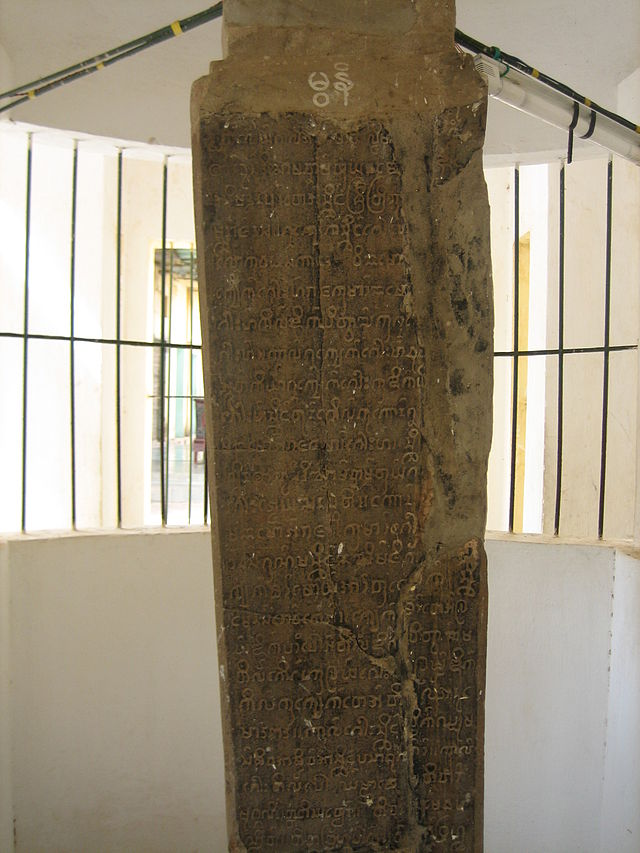
\includegraphics[width=\linewidth, height=3.5cm]{./fig/myasadi.jpg}
    \caption{{\padauktext မြစေတီကျောက်စာ \\ (မွန်ကျောက်စာ)}}
  \end{subfigure}
  \begin{subfigure}[b]{0.4\linewidth}
    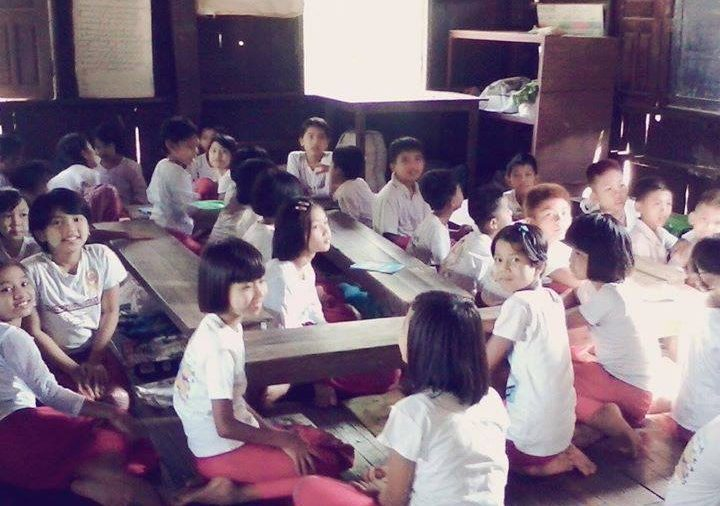
\includegraphics[width=\linewidth, height=3.5cm]{./fig/monsarpay.jpg}
    \caption{{\padauktext မွန်စာပေသင်တန်းများ\\ဖွင့်လှစ်သင်ကြားပုံ}}
  \end{subfigure}
  \begin{subfigure}[b]{0.4\linewidth}
    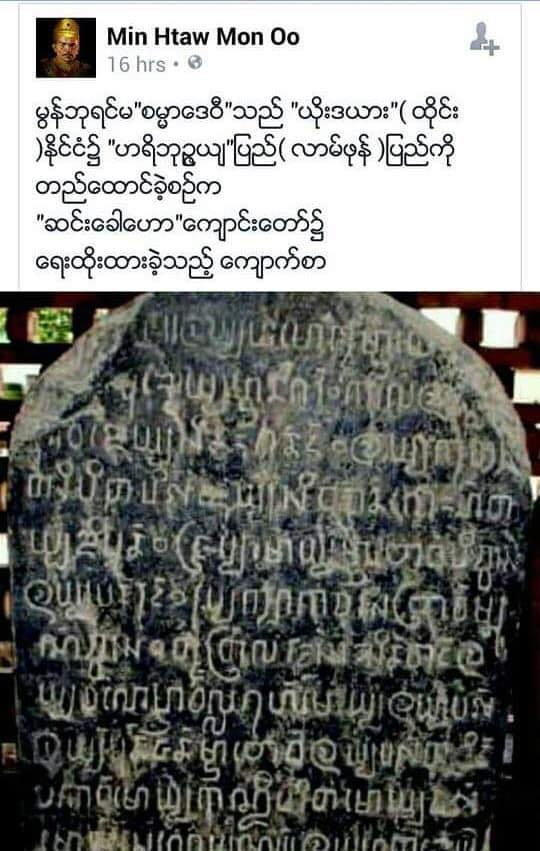
\includegraphics[width=\linewidth, height=3.5cm]{./fig/bagan.jpg}
    \caption{{\padauktext ဆင်ခေါဟောကျောင်းတိုက်\\၌ ရေးထိုးခဲ့သည့်မွန်ကျောက်စာ}}
  \end{subfigure}
  \begin{subfigure}[b]{0.4\linewidth}
    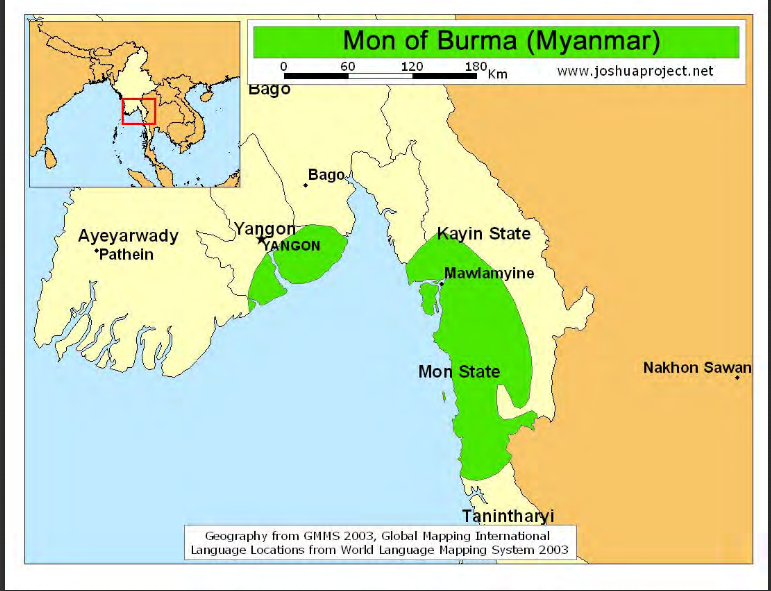
\includegraphics[width=\linewidth, height=3.5cm]{./fig/mon-bruma.png}
    \caption{{\padauktext မြန်မာနိုင်ငံ ရှိ မွန်စာပေ \\ ထွန်းကားရာနေရာ}}
  \end{subfigure}
  \caption{Mon Language of learning (11th-12th century)}
  \label{fig:mon}
\end{figure}

\section{Conclusion}
The Mon language and people are one of the first to appear in the documented history of Southeast Asia. Being in close contact with peoples speaking languages vastly different from their own, they were both donors and recipients of linguistic features crossing the language boundaries. Mon serves as a good playground for contact linguistics, as it has been the source and goal of contact induced changes under influence from languages of a very different typological profile, such as Burmese, as well as the typologically much more similar Thai and others. 
\par The contact induced changes in Mon, Burmese and Thai are the most accessible as they involve languages
with a long recorded history. Much less is known about convergence with other languages in the area, especially Karen varieties, some of which are known to be heavily influenced by Mon, such as eastern Pwo. Maybe the general SVO constituent order of Karen languages can be attributed to Mon-Khmer or perhaps Mon influence, but much more research is needed in this area. In this paper I only attempted to give a general overview of the contact phenomena found in Mon and the two large neighbouring languages. Future in-depth research in the field with more reliable data from hitherto ill-described languages will certainly add to our understanding of the
linguistic (and social) landscape of western Southeast Asia, both past and present.

\begin{thebibliography}{00}

\bibitem{b1} https://www.omniglot.com/writing/mon.html
\bibitem{b2} https://www.albany.edu/~gb661/monhist1.html
\bibitem{b3} https://en.wikipedia.org/wiki/Mon\_language\#Dialects
\bibitem{b4} TheMonLanguageInThailandAndMyanmarMJ2015.pdf. Receivedfrom: http://www.comparativelinguistics.uzh.ch/staff/mathiasjenny/download
\bibitem{b5} https://en.wikipedia.org/wiki/Mon\_language\#Consonants
\bibitem{b6} https://sites.google.com/a/mondhamma.com/mon-dhamma/home/mon-alphabet-and-grammer
\bibitem{b7} https://en.wikipedia.org/wiki/Mon\_language\#Phonology
\bibitem{b8} https://en.wikipedia.org/wiki/Mon\_language\#Vocalic\_register
\bibitem{b9} Mathias Jenny, The Mon language:recipient and donor between Burmese and Thai
\bibitem{b10} Mathias Jenny, 2000 years of history \- the Mon language in Thailand and Myanm

\end{thebibliography}
%\vspace{12pt}
%\color{red}
%IEEE conference templates contain guidance text for composing and formatting conference papers. Please ensure that all template text is removed from your conference paper prior to submission to the conference. Failure to remove the template text from your paper may result in your paper not being published.

\end{document}
